\chapter{AppVeyor}

AppVeyor是一个由加拿大成立于2011年的持续集成项目,并于2013年提供公开服务。
该平台最初的目标面向Windows项目,是早年免费为开源项目提供Windows持续集成服务的项目之一。

由于AppVeyor可以追踪GitHub中的提交,并对开源项目免费提供单线程的持续集成,
是很多开源项目选择的持续集成工具之一。通过AppVeyor,可以很方便的获取项目产出文件,
同时在合并分支前对代码兼容性进行初步检查,发现无法通过编译的合并请求。

使用AppVeyor,首先需要创建新项目。可以看到,AppVeyor支持几乎所有的主流的基于Git的代码管理平台,
包括使用Git协议的私人平台,因此很容易集成。选择项目后,AppVeyor会监控该项目,并在满足集成条件时
使用项目最新的代码进行集成,并给出项目产物,免去了开发人员和使用者需要手动编译的麻烦。

\begin{figure}[h]
    \centering
    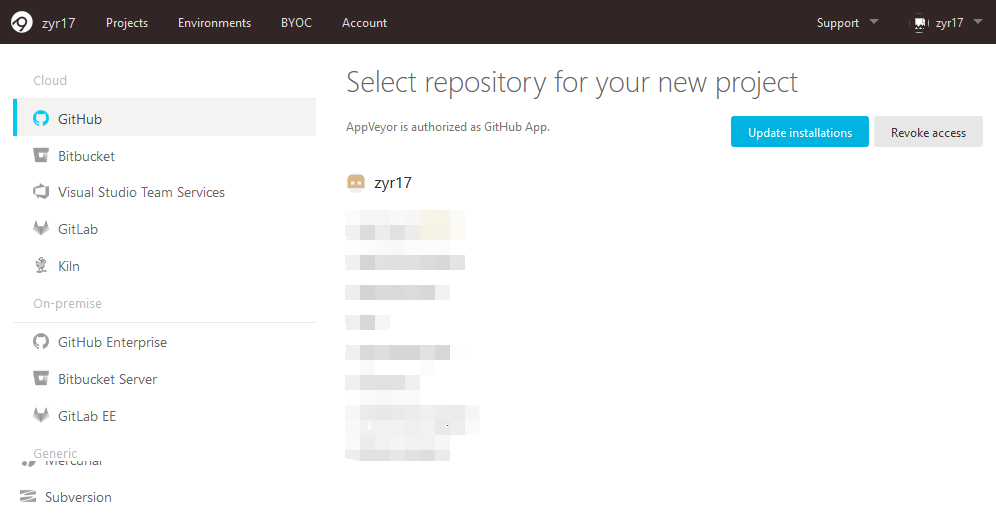
\includegraphics[width=1\textwidth]{figures/appveyor/create.png}
    \caption{创建新AppVeyor项目}
    \label{fig:appveyor_create}
\end{figure}

最方便的使用AppVeyor的方法是在项目中添加appveyor.yml,AppVeyor会自动读取该文件并根据文件中的
配置和命令进行自动集成。我们也可以手动对项目进行设置,例如指定其他名称的配置文件,
或者将配置文件写于AppVeyor上而非读取代码库中的配置文件。

以某个项目的配置文件为例,本文会对AppVeyor的项目配置做简要介绍。

\begin{figure}[h]
    \centering
    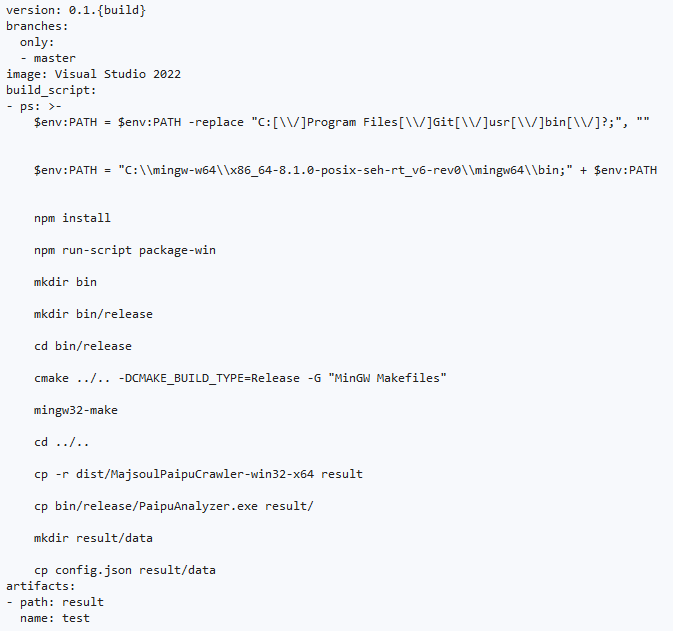
\includegraphics[width=1\textwidth]{figures/appveyor/config.png}
    \caption{AppVeyor配置文件}
    \label{fig:my_label}
\end{figure}

首先配置中需要指定每次集成的版本号。由于需要保证每次的版本号不一样,所以包含一个
每次集成后自增1的build。然后需要指定在什么情况下触发自动集成,这里的设置是
仅当master分支有新的commit时触发。接下来是指定运行环境,这里的Visual Studio 2022
并非单指该IDE,而代表了以Visual Studio为主的一系列环境。显然,这是一个Windows环境,
用于编译Windows项目,AppVeyor目前也提供Linux和Mac项目的持续集成服务。在build\_script
中,是集成时需要执行的命令。在该配置中,使用了PowerShell作为集成命令行。同时,
AppVeyor对脚本的设置类似markdown,除非连续两个换行符,否则将多行脚本看成单行脚本,
这样便于在配置中编写较长的脚本,但也会增加多行脚本的行数。最后,在持续集成完成后,
使用artifacts指定产物目录和文件名,这样就能够在验证代码有效性的同时直接获取构建产物。

AppVeyor作为早期平台,其易用性较高,但是支持较为单一,由于底层基于虚拟机实现,
工作流类似于在一台服务器上进行编译,较难实现复杂的控制流和多任务,
目前在开源社区用于用于自动构建产物较多。